\section{GUI}

\subsection{Indledning}
Da et af de sekundære mål var at afsende billeder, ville det være fordelagtigt at bruge en grafisk brugerflade istedet for konsollen, da det ville gøre det muligt at se billedet direkte i den grafiske brugerflade.

Da der ingen undervisning i grafiske brugerflader har været dette semester, blev der valgt en udviklingsplatform kaldet QT til at lave den grafiske brugerflade.
Valget stod mellem QT, Windows forms, og Python.
Da QT var det første som blev undersøgt, og virkede meget ligetil, var det det som blev valgt.
QT er et program som er bygget op om C++ syntax, er brugervenligt og let at lære at skrive, hvis C++ allerede er et kendt programmeringssprog.\\
\subsection{Funktionalitet}

I den grafiske brugerflade er der 3 elementer.
\begin{itemize}[noitemsep]
	\item Chat boks: hvori selve chatten foregår, her kommer der til at stå hvad der modtages, samt hvilket input der gives.
	\item Send knap: denne afsender den tekst som er skrevet i chat linjen.
	\item Chat linje: dette er hvor input fra brugeren kommer til at stå, når der skrives noget. Det er dette der bliver sendt når det bliver trykket på enter / send knappen.
\end{itemize}

Når der skrives noget i chat linjen, og der trykkes på enter / send knappen, kaldes en funktion fra applikationslaget som hedder send. Den tager som parameter strengen fra inputlinjen.

\subsection{Delkonklussion}
Den grafiske brugerflade blev valgt til at være et helt standard chatvindue som set på figur \ref{fig:GUI}.
Brugerfladen blev ikke implementeret da der var problemer med at holde en sideløbende tråd kørende samtidig med brugerfladen.
Dette blev opdaget for sent og da der var ikke tid til at fejlfinde, blev alternativet konsollen valgt.
Samtidig var målet med at afsende billeder ikke blevet nået så den grafiske brugerflade var ikke nødvendig.

\begin{figure}[h!]
\centering
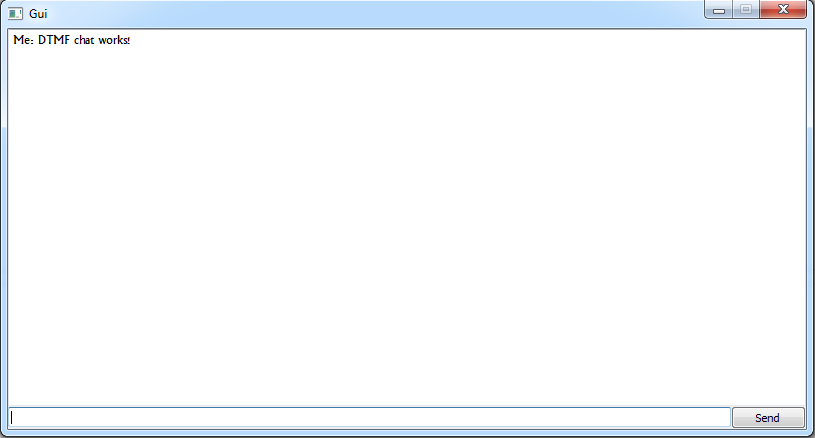
\includegraphics[scale=0.5]{Billeder/GUI.PNG}
\caption{Her ses den grafiske brugerflade}
\label{fig:GUI}
\end{figure}